\section{Penelitian Terkait}
Pada sub-bab ini, dibahas beberapa penelitian yang telah dilakukan terhadap pemanfaatan metode PEFT.

\subsection{UniPELT}

Setiap metode PEFT yang yang telah dijelaskan pada subbab-subbab sebelumnya mempunyai karakteristik yang beragam dan memiliki kinerja yang cukup berbeda pada tugas yang sama \parencite{unipelt}. Sehingga, pemilihan metode PEFT yang paling tepat untuk tugas tertentu menjadi tugas yang cukup sulit, terutama dengan jumlah metode PEFT yang terus bertambah \parencite{unipelt}. UniPELT hadir sebagai \textit{framework} yang menyatukan beberapa metode PEFT sebagai submodul dan mencoba belajar untuk menggunakan metode PEFT yang terbaik pada suatu tugas \parencite{unipelt}.

UniPELT menggunakan empat metode yang cukup merepresentasikan banyakanya metode PEFT, yaitu \textit{Adapter}, \textit{Prefix-Tuning}, LoRA, dan BitFit \parencite{unipelt}. Semua metode tersebut sudah dibahas pada subbab sebelumnya, kecuali BitFit. BitFit merupakan metode PEFT yang hanya melakukan pelatihan pada bias dari modelnya saja \parencite{unipelt}. Berdasarkan eksperimen yang dilakukan oleh \citeauthor{unipelt}, BitFit tidak pernah mendapatkan hasil yang terbaik dan secara umum mendapatkan hasil yang terburuk, sehingga BitFit tidak dimasukkan ke dalam metode gabungan dari UniPELT dan hanya digunakan sebagai pembanding pada eksperimen \parencite{unipelt}.

\begin{figure}[h]
    \vspace{0.25cm}
    \centering
    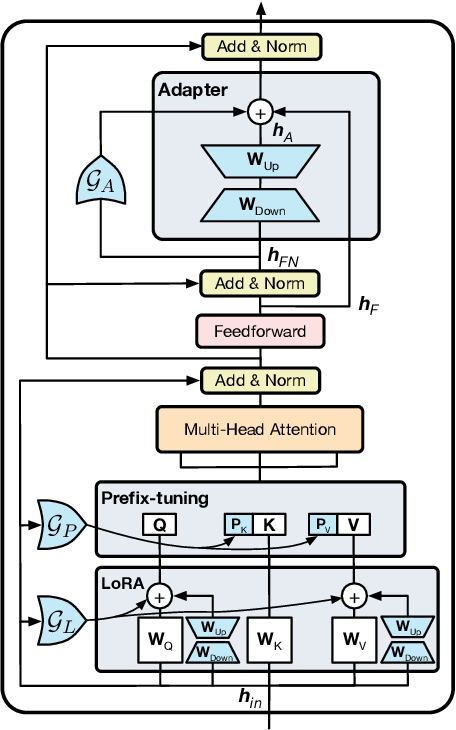
\includegraphics[height=0.4\textheight]{chapter-2/unipelt_arch.png}
    \caption{Arsitektur UniPELT \parencite{unipelt}}
    \label{fig:unipelt_arch}
\end{figure}

Setiap metode PEFT menggunakan bagian yang berbeda pada arsitektur model, sebagai contoh sebelum \textit{multi-head attention} untuk \textit{Prefix-Tuning} dan setelah \textit{feed-forward} untuk \textit{Adapter} \parencite{unipelt}. Sehingga, memungkinkan untuk menggabungkan beberapa metode PEFT tersebut tanpa mengganggu antara satu metode dengan yang lain \parencite{unipelt}. Arsitektur dari gabungan metode PEFT tersebut dapat dilihat pada gambar \ref{fig:unipelt_arch}. Selain menggabungkan, terdapat \textit{gating mechanism} yang akan melakukan aktivasi atau deaktivasi tergantung dari signifikasi kinerja setiap metode PEFT pada tugas yang sedang dilatih \parencite{unipelt}.

\citeauthor{unipelt} melakukan eksperimen dengan \textit{low-resource} dan \textit{high-resource} pada evaluasi GLUE dengan menggunakan model BERT \parencite{unipelt}. Metode UniPELT divariasikan menjadi dua yaitu UniPELT (AP) dan UniPEL (APL), dengan $A$ berarti \textit{Adapter}, $P$ berarti \textit{Prefix-Tuning}, dan $L$ berarti LoRA. Secara umum, UniPELT (AP) dan UniPELT (APL) secara konsisten mendapatkan hasil yang terbaik atau kedua terbaik pada rata-rata evaluasi GLUE untuk semua eksperimen \textit{low-resource} \parencite{unipelt}. Kinerja UniPELT lebih baik dibanding dengan masing-masing submodulnya upada eksperimen \textit{low-resource}, yang menunjukkan bahwa UniPELT menghasilkan kinerja yang baik untuk eksperimen tersebut \parencite{unipelt}.

Perhitungan parameter untuk UniPELT merupakan total dari metode sebelumnya. Namun, terdapat \textit{gating mechanism} yang merupakan fungsi linear untuk melakukan aktivasi atau deaktivasi pada setiap metode PEFT terkait. Rumus \ref{eq:parameter-prefix-tuning} menunjukkan perhitungan untuk parameter pelatih dengan $A$, $P$, dan $L$ adalah metode \textit{Adapter}, \textit{Prefix-Tuning}, dan LoRA. Seperti yang bisa dilihat pada rumus \ref{eq:parameter-prefix-tuning}, $gating$ merupakan fungsi linear yang terkait terhadap $d_{hidden}$. Terdapat perbedaan dari pengali pada $gating_{P}$ dari rumus \ref{table:param-model}, modul \textit{prefix} dianggap sebagai 1 untuk kedua $key$ dan $value$.

\begin{equation}
    \begin{aligned}
        gating = d_{hidden} \times 1 + 1 \\
        gating_{A} = gating \times block \times forward\_head \\
        gating_{P} = gating \times block \times attention\_head \\
        gating_{L} = gating \times 2 \times block \times attention\_head \\
        total\_gating = (3 \times attention\_head + forward\_head) \times gating \times block \\
        \psi = \psi_A + \psi_P + \psi_L + total\_gating
    \end{aligned}
    \label{eq:parameter-unipelt}
\end{equation}

\begin{table}[ht]
    \vspace{0.25cm}
    \centering
    \caption{Hasil evaluasi UniPELT pada \textit{high-resource} \parencite{unipelt}}
    \label{table:unipelt_result}
    \resizebox{\textwidth}{!}{
        \begin{tabular}{l|ccccccccccc}
            \toprule
            Method & SST-2 & MRPC & CoLA & RTE & QNLI & STS-B & MNLI & QQP & Avg. \\
            \midrule
            Fine-tuning & 91,63 & 90,94 & 62,08 & 66,43 & 89,95 & \textbf{89,76} & 83,23 & \textbf{87,35} & 82,67 \\
            Adapter & \textbf{91,86} & 89,86 & 61,51 & 71,84 & 90,55 & 88,63 & 83,14 & 86,78 & 83,02 \\
            Prefix-tuning & 90,94 & \textbf{91,29} & 55,37 & \textbf{76,90} & 90,39 & 87,19 & 81,83 & 82,30 & 82,07 \\
            LoRA & 91,51 & 90,03 & 60,47 & 71,48 & 90,73 & 85,65 & 85,61 & 85,98 & 82,20 \\
            \midrule
            UNIPELT (AP) & \textbf{91,86} & 90,28 & 61,51 & 71,84 & \textbf{90,77} & \textbf{88,76} & 83,12 & 86,78 & 83,02 \\
            -NoGate & 91,74 & 90,18 & 58,63 & 71,12 & 90,38 & 88,76 & 81,54 & 85,83 & 82,23 \\
            UNIPELT (APL) & 91,51 & 90,94 & 61,53 & 73,65 & 90,50 & 88,93 & \textbf{83,89} & 87,12 & \textbf{83,50} \\
            \bottomrule
        \end{tabular}
    }
\end{table}

Pada tabel \ref{table:unipelt_result} merupakan hasil evaluasi dari UniPELT pada \textit{high-resource}, UniPELT mendapatkan hasil yang terbaik secara umum. Peningkatan yang didapatkan tidak terlalu signifikan dibandingkan dengan eksperimen pada \textit{low-resource}, hal ini sesuai karena metode PEFT mampu menyaingi \textit{fine-tuning} pada \textit{dataset} yang banyak \parencite{unipelt}. Hasil UniPELT tanpa dilakukan \textit{gating mechanism} (-NoGate) tidak menghasilkan kinerja yang baik \parencite{unipelt}. Walaupun dengan kinerja yang baik, \citeauthor{unipelt} menyebutkan bahwa penggunaan UniPELT tidak akan selalu menghasilkan hasil yang lebih baik dibandingkan dengan penggunaan submodulnya secara individual, bahkan bisa memberikan hasil yang lebih buruk \parencite{unipelt}.

\begin{table}[ht]
    \vspace{0.25cm}
    \centering
    \caption{Waktu pelatihan dan inferensi dari setiap metode PEFT \parencite{unipelt}}
    \label{table:runtime-peft}
    \begin{tabular}{lrrr}
        \toprule
        \textbf{Method} & \textbf{\#Param.} & \textbf{Time$_T$} & \textbf{Time$_I$} \\ 
        \midrule
        Fine-tuning & 110M (100\%) & 100\% & 100\% \\ 
        BitFit & 103K (0,09\%) & 65\% & 102\% \\ 
        Prefix-tuning & 184K (0,17\%) & 56\% & 114\% \\ 
        LoRA & 295K (0,27\%) & 53\% & 105\% \\ 
        Adapter & 895K (0,81\%) & 55\% & 107\% \\ 
        UNIPELT (AP) & 1,1M (0,99\%) & 55\% & 118\% \\ 
        UNIPELT (APL) & 1,4M (1,26\%) & 67\% & 127\% \\ 
        \bottomrule
    \end{tabular}
\end{table}

Pada penelitian yang dilakukan oleh \citeauthor{unipelt}, dilakukan juga evaluasi terhadap waktu pelatihan dan waktu inferensi antara masing-masing metode PEFT, seperti yang bisa dilihat pada tabel \ref{table:runtime-peft}. Waktu pelatihan yang didapatkan dengan metode PEFT lebih cepat dibandingkan dengan \textit{fine-tuning} karena parameter yang digunakan untuk pelatihan juga lebih sedikit \parencite{unipelt}. Untuk waktu inferensi, semuanya menjadi lebih besar dibandingkan dengan \textit{fine-tuning} karena metode PEFT membutuhkan \textit{floating-point operations per second} (FLOPS) yang lebih besar \parencite{unipelt}.

\subsection{\textit{Parameter-Efficient Fine-Tuning of Large-Scale
Pre-Trained Language Models}}

Penelitian yang dilakukan oleh \citeauthor{peft_on_plm} membandingkan secara komprehensif terkait metode \textit{transfer-learning} yang efisien secara parameter pada \textit{pre-trained model}. Metode ini disebut sebagai \textit{delta-tuning} pada penelitian tersebut, dengan kata 'delta' muncul dari notasi matematika yang merepresentasikan perubahan \parencite{peft_on_plm}. Metode \textit{delta-tuning} yang digunakan adalah \textit{prompt-tuning} (PT), \textit{prefix-tuning} (PF), LoRA (LR), dan \textit{adapter} (AP). \textit{Delta-tuning} tersebut  dibandingkan dengan \textit{fine-tuning} (FT) .

Eksperimen yang dilakukan pada penelitian tersebut dilakukan pada model T5 dengan konfigurasi BASE dan LARGE. Evaluasi metode \textit{delta-tuning} pada model T5 dilakukan pada 100 tugas pemrosesan bahasa alami yang diambil dari \textit{dataset} Huggingface. Tugas yang dipilih termasuk \textit{text classification}, \textit{question answering}, dan \textit{generation}.

Berdasarkan hasil yang didapatkan pada eksperimen tersebut, metode \textit{delta-tuning} dengan pengurangan jumlah parameter yang dilatih dibandingkan dengan \textit{fine-tuning} memberikan hasil yang hampir setara pada sebagian besar tugas. Metode \textit{prefix-tuning}, LoRA, dan \textit{adapter} secara kinerja hampir mirip antara satu sama lain. Bahkan, metode \textit{delta-tuning} pada sebagian tugas mampu memberikan hasil yang dominan dibanding \textit{fine-tuning}. Secara keseluruhan, kinerja pada setiap metode dapat diurutkan sebagai berikut.

\begin{enumerate}
    \item \textit{Fine-Tuning} (FT)
    \item \textit{Low-Rank Adaptation} (LoRA)
    \item \textit{Adapter Tuning} (AP)
    \item \textit{Prefix Tuning} (PF)
    \item \textit{Prompt Tuning} (PT)
\end{enumerate}

\begin{figure}[ht]
    \centering
    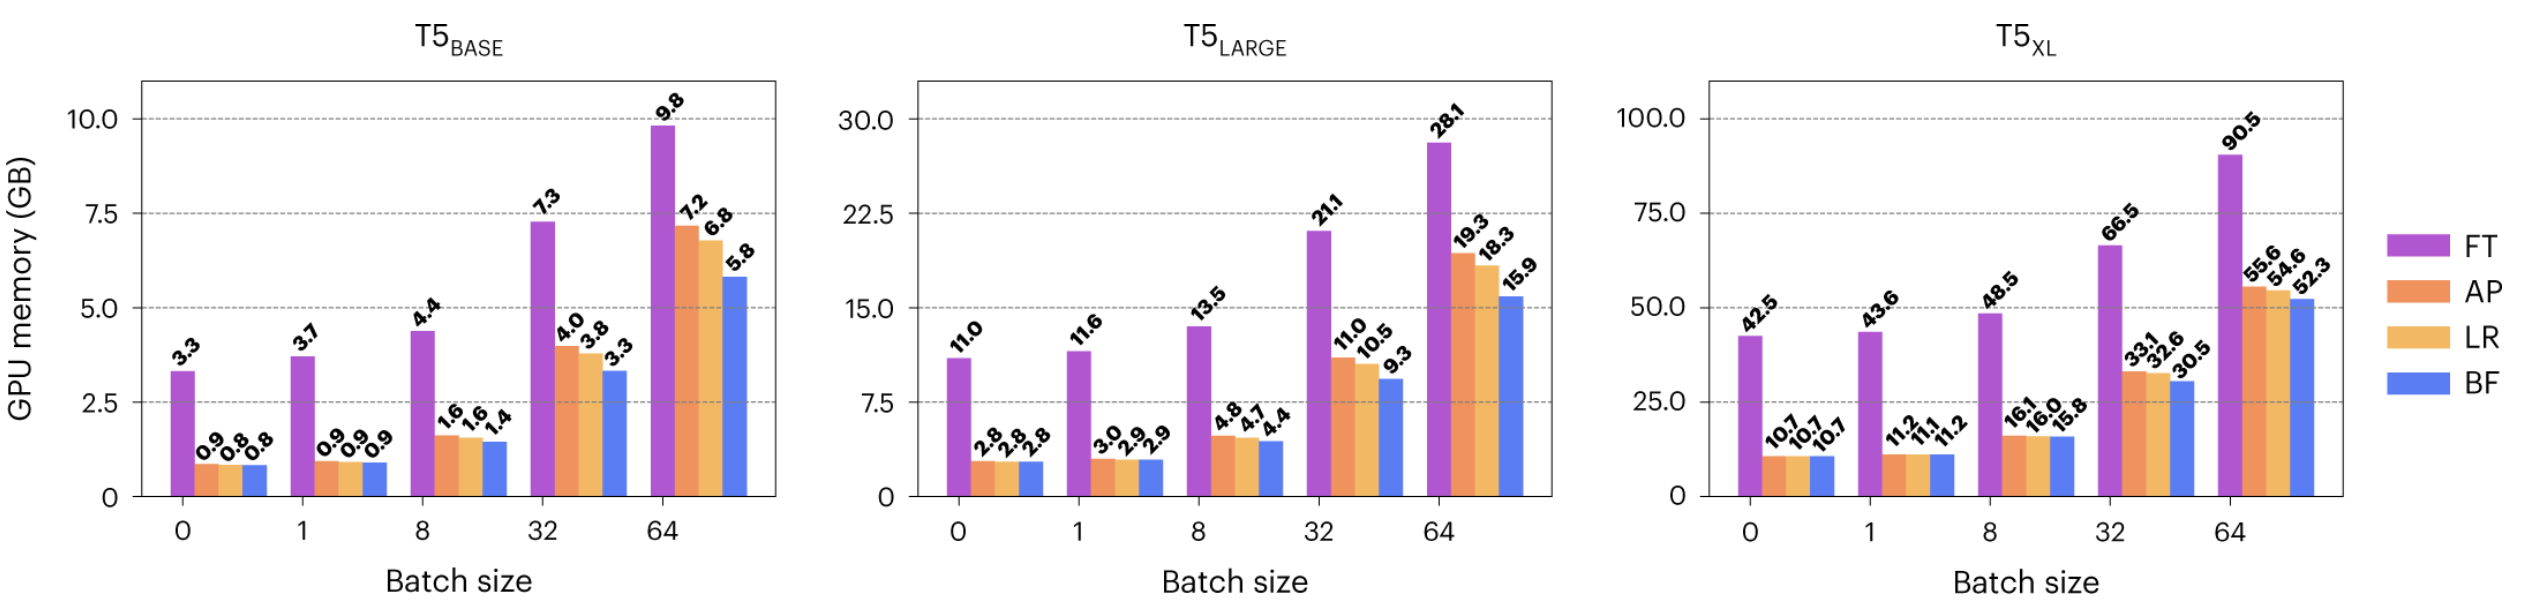
\includegraphics[width=1\textwidth]{chapter-2/peft_on_plm_memory.png}
    \caption{Perbandingan Efisiensi Memori \parencite{peft_on_plm}}
    \label{fig:peft_on_plm_memory}
\end{figure}

Selain itu, dilakukan juga eksperimen terkait analisis pada efisiensi dari tiap metode. Eksperimen ini mengeksplorasi penggunaan efisiensi memori GPU pada metode \textit{delta-tuning} dan FT pada model T5 dengan konfigurasi BASE, LARGE, dan XL. Metode \textit{delta-tuning} yang digunakan adalah LoRA (LR), dan \textit{adapter} (AP), dan BitFit (BF). Berdasarkan Gambar \ref{fig:peft_on_plm_memory}, penggunaan memori pada setiap metode \textit{delta-tuning} berkurang dibandingkan dengan \textit{fine-tuning}. Hasil ini menunjukkan bahwa \textit{delta-tuning} mengurangi penggunaan memori GPU dengan mengurangi kebutuhan komputasi gradien untuk mengubah parameter \parencite{peft_on_plm}.

